% Source: Lecture11.pdf, pages 1-6.
\lecture{11}
\subsubsection*{Mean field theory for an \texorpdfstring{$O(2)$}{O(2)} spin model}

An example of an application of mean field theory to a continuous spin system: consider a spin
model with spins in $S^1$, i.e.\ $\mathbf{S}_i = (\cos\theta_i,\sin\theta_i)$ (normalize
$\mathbf{S}$ so $|\mathbf{S}| = 1$), and
\begin{equation}
  \Ham = -J\sum_{e_{ij}}\mathbf{S}_i\cdot\mathbf{S}_j - \mathbf{H}\cdot\sum_i\mathbf{S}_i .
\end{equation}
The spin--spin interaction is
\begin{equation}
  \mathbf{S}_i\cdot\mathbf{S}_j = \cos\theta_i\cos\theta_j + \sin\theta_i\sin\theta_j = \cos(\theta_i-\theta_j).
\end{equation}
In the absence of an external magnetic field $\mathbf{H}$, the Hamiltonian is invariant under a
global $O(2)$ symmetry group with elements $R(\omega)$ that rotate each spin by the angle $\omega$.
This is clear, since the scalar product $\mathbf{S}_i\cdot\mathbf{S}_j$ is invariant under such
rotations: $\cos(\theta_i-\theta_j)\to\cos((\theta_i+\omega)-(\theta_j+\omega))$. A nonzero external
field breaks this $O(2)$ symmetry explicitly and a nonzero spontaneous magnetization breaks it
spontaneously. The partition function is now the multiple ($N$-fold) integral
\begin{equation}
  Z = \left[\prod_{i=1}^N\int_0^{2\pi}\frac{\dd\theta_i}{2\pi}\right]e^{-\beta\Ham}
    = \left[\prod_{i=1}^N\int_0^{2\pi}\frac{\dd\theta_i}{2\pi}\right]
      e^{K\sum_{e_{ij}}\cos(\theta_i-\theta_j) + h\sum_i\cos\theta_i},
\end{equation}
where we have taken $\mathbf{H}$ to point along the $\hat{\mathbf{x}}$ axis in the $O(2)$ space (just
define $\hat{\mathbf{x}}$ in $O(2)$ space to point along $\mathbf{H}$; no loss of generality).

MFT approximates the partition function by assuming that each spin interacts with a mean field (per
site) $\bar{\mathbf{M}}\equiv\langle\mathbf{M}\rangle$ due to all of the other spins, so the full
partition function reduces to an $N$-fold product of single-site (ss) integrals. Since
$\mathbf{H} = H(1,0)$, the induced $\bar{\mathbf{M}} = \bar M(1,0)$. So for the reference spin
$\mathbf{S}_0$,
\begin{equation}
  \sum_{e_{0j}}\mathbf{S}_0\cdot\ev{\mathbf{S}} = (\cos\theta_0,\sin\theta_0)\cdot\bar M(1,0)\,\Delta
  = (\bar M\cos\theta_0)\,\Delta,
\end{equation}
where $\Delta$ = lattice coordination number, and $Z_{\text{MFT}} = (Z_{ss})^N$, with
\begin{equation}
  Z_{ss} = \int_0^{2\pi}\frac{\dd\theta_0}{2\pi}e^{K\sum_{e_{0j}}\mathbf{S}_0\cdot\ev{\mathbf{S}} + \mathbf{h}\cdot\mathbf{S}_0}
  = \int_0^{2\pi}\frac{\dd\theta_0}{2\pi}e^{(K\Delta\bar M+h)\cos\theta_0},
  \qquad x\equiv K\Delta\bar M + h .
\end{equation}
Now
\begin{equation}
  \int_0^{2\pi}\frac{\dd\theta_0}{2\pi}e^{x\cos\theta_0} = I_0(x),
\end{equation}
where $I_\nu(x)$ is the modified Bessel function of index $\nu$, with series expansion
\begin{equation}
  I_\nu(x) = \sum_{\ell=0}^\infty\frac{(x/2)^{\nu+2\ell}}{\ell!\,\Gamma(\nu+\ell+1)},
\end{equation}
where $\Gamma(y)$ is the Euler $\Gamma$ function: $\Gamma(y+1) = y\Gamma(y)$ and $\Gamma(n) = (n-1)!$
for integer $n$. So
\begin{gather}
  I_0(x) = 1 + \frac{(x/2)^2}{\Gamma(2)} + \Order(x^4) = 1 + \frac{x^2}{4} + \Order(x^4)
  \quad(\Gamma(2) = 1),\nonumber\\
  I_1(x) = \frac{(x/2)}{\Gamma(2)} + \Order(x^3) = \frac{x}{2} + \Order(x^3).
\end{gather}
Another relation is $\dd I_0(x)/\dd x = I_1(x)$. The dimensionless reduced Gibbs free energy in
the MFT approximation is then
\begin{equation}
  f_{\text{MFT}} = \lim_{N\to\infty}\frac{1}{N}\ln Z_{\text{MFT}} = \ln(Z_{ss}) = \ln(I_0(x)) = \ln\left[I_0(K\Delta\bar M+h)\right].
\end{equation}
Calculate $\bar M$:
\begin{equation}
  \bar M = \pder{f}{h} = \pder{}{h}\ln\left[I_0(K\Delta\bar M+h)\right] = \frac{I_1(K\Delta\bar M+h)}{I_0(K\Delta\bar M+h)}.
\end{equation}
The spontaneous magnetization is $\bar M_{sp} = \lim_{h\to 0}\bar M$, so
\begin{equation}
  \bar M_{sp} = \frac{I_1(K\Delta\bar M_{sp})}{I_0(K\Delta\bar M_{sp})}.
\end{equation}
This is the analogue, in this $O(2)$ spin model, of the equation
$\bar M_{sp} = \tanh(K\Delta\bar M_{sp})$ that we derived previously for the Ising model in the MFT
approximation. As before, at high temperature $T$, i.e.\ small $\beta$ and hence small $K = \beta J$,
the only solution is $\bar M_{sp} = 0$. As $T$ decreases, and hence $K$ increases, a nonzero solution
first occurs if RHS $=\bar M_{sp}$, where $|\bar M_{sp}|\ll 1$. So we calculate this by expanding the
Bessel functions for small arguments, using $I_1(x) = x/2 + \Order(x^3)$ and
$I_0(x) = 1 + \Order(x^2)$:
\begin{equation}
  \bar M_{sp} = \frac{K\Delta\bar M_{sp}}{2} + \ldots,
\end{equation}
so a nonzero solution occurs as $K$ is increasing from 0 at $K\Delta = 2$, i.e.
\begin{equation}
  K = K_{c,\text{MFT},O(2)} = \frac{2}{\Delta}.
\end{equation}
Comparing this with the result for Ising, $K_{c,\text{MFT},\text{Ising}} = 1/\Delta$, we see that
\begin{equation}
  \kB T_{c,\text{MFT},O(2)} = \frac{J\Delta}{2}\qquad\text{vs.}\qquad\kB T_{c,\text{MFT},\text{Ising}} = J\Delta .
\end{equation}
So MFT predicts that one must cool a system of $O(2)$ spins to twice as low a temperature to get the
phase transition to the symmetry-broken phase with a spontaneous magnetization as compared with an
Ising spin model on the same lattice. This is physically understandable because the spins in the
$O(2)$ model are ``floppier'' than the spins in the Ising model, so one needs a lower temperature to
get them to have ``long-range order'' (LRO), where ``long'' means infinite.

Thus, MFT yields predictions for $T_c$ that depend on
\begin{enumerate}[label=(\roman*)]
  \item the lattice coordination number (vertex degree) $\Delta$;
  \item intrinsic properties of the dynamical variables, as shown e.g.\ by the comparison of the
    application to the Ising vs.\ $O(2)$ spin models;
  \item because of the neglect of fluctuations in MFT, the true $T_c$ is smaller than the MFT
    prediction.
\end{enumerate}
We showed this quantitatively by comparing the MFT prediction for $T_c$ with the exactly known
$T_c$ for the Ising model on a 2D lattice (the square lattice) and two 3D lattices, sc and bcc. We
saw that the MFT prediction becomes more accurate as the dimension of the lattice increases.

A drastic example of a failure of MFT is for a 1-dimensional lattice. Here, $\Delta = 2$, so MFT
predicts that there will be a phase transition to a ferromagnetic phase at a finite temperature,
e.g.\ $T_c = J\Delta/\kB = 2J/\kB$ for an Ising model. But the Peierls Theorem shows that there is no
nonzero spontaneous magnetization and associated FM LRO at any finite temperature; this only occurs
at $T = 0$. Our exact solution for $\bar M(T,H)$ and $\bar M_{sp} = \lim_{H\to 0}\bar M(T,H)$ showed
this explicitly.

\subsection{Peierls argument in two and more dimensions}

Recall the Peierls Theorem for a 1D spin system, e.g.\ Ising. This showed that a would-be
ferromagnetically ordered state is unstable to the occurrence of a disordering seam (and hence to
multiple such seams), from $\cdots{+}{+}{+}{+}{+}{+}\cdots$ to $\cdots{+}{+}{+}\,|\,{-}{-}{-}\cdots$,
with a seam where the spins flip:
\begin{equation}
  \Delta G = 2J - T\Delta S = 2J - \kB T\ln N,
\end{equation}
since the seam can occur anywhere. As $N\to\infty$, for any $T>0$, the second term dominates, so
the occurrence of this disordering seam lowers the free energy. Only at $T = 0$, where
$\Delta G = \Delta U$, does the seam raise the free energy, and hence only at $T = 0$ does the system
have $\bar M\ne 0$.

We now show how a Peierls-type argument proves that for a discrete spin model in $d\ge 2$
dimensions (without frustration or competing interactions) there is a phase transition to a
low-temperature phase with nonzero spontaneous magnetization. Consider the FM case $J>0$; on a
bipartite lattice there is an isomorphism relating this to the AFM case $J<0$. Consider a
ferromagnetically ordered state, and again analyze $\Delta G$ when one introduces a disordering
seam, e.g.\ on the square lattice.

\begin{diagram}
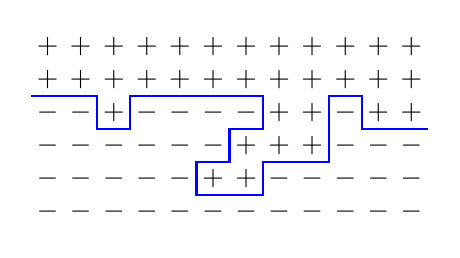
\begin{tikzpicture}[scale=0.42]
  \foreach \r/\row in {
    0/{+,+,+,+,+,+,+,+,+,+,+,+},
    1/{+,+,+,+,+,+,+,+,+,+,+,+},
    2/{-,-,+,-,-,-,-,+,+,-,+,+},
    3/{-,-,-,-,-,-,+,+,+,-,-,-},
    4/{-,-,-,-,-,+,+,-,-,-,-,-},
    5/{-,-,-,-,-,-,-,-,-,-,-,-}} {
    \foreach \s [count=\c] in \row { \node at (\c,-\r) {$\s$}; } }
  \draw[blue,thick] (0.5,-1.5) -- (2.5,-1.5) -- (2.5,-2.5) -- (3.5,-2.5) -- (3.5,-1.5) -- (7.5,-1.5)
     -- (7.5,-2.5) -- (6.5,-2.5) -- (6.5,-3.5) -- (5.5,-3.5) -- (5.5,-4.5) -- (7.5,-4.5) -- (7.5,-3.5)
     -- (9.5,-3.5) -- (9.5,-1.5) -- (10.5,-1.5) -- (10.5,-2.5) -- (12.5,-2.5);
\end{tikzpicture}
\diagramcaption{A disordering seam (blue) in a rectangular section of an $n\times n$ square
lattice, so $N_{\text{tot}} = n^2$. The increase in the internal energy is $(2J)L$, where $L$ is
the length of the seam.}
\end{diagram}

Now make rough estimates of typical lengths $L$ and the entropic term $T\Delta S$ to estimate the
$\Delta G$ due to the seam. Say we start the wall from the left; there are $\sim n$ places where it
can start. At a typical internal site, there are at least 2 ways, and sometimes 3 ways, the seam
can propagate ($\rightarrow\rightarrow$ or $\rightarrow\uparrow$ or $\rightarrow\downarrow$). Let us
denote this number of choices as $c$, where $2\le c\le 3$. Since the seam zigzags, its length
$L>n$; use the estimate $L\simeq\lambda n$. Then the change in the internal energy $U$ due to the
seam is
\begin{equation}
  \Delta U = (2J)L\simeq 2J\lambda n .
\end{equation}
Since the seam can start at any of $n$ positions on the left and since at every step there are $c$
choices of how to proceed, the entropic term is
\begin{equation}
  -T\Delta S\simeq -\kB T\ln(n\cdot c^L) = -\kB T\ln\left(n\cdot e^{\lambda n\ln c}\right)
  = -\kB T\left[\ln n + \lambda n\ln c\right];
\end{equation}
for $n\gg 1$ the term $\propto n$ dominates over the $\ln n$ term, which we can drop. So
\begin{equation}
  \Delta G\simeq 2J\lambda n - \kB T\cdot\lambda n\ln c = \lambda n(2J - \kB T\cdot\ln c),
  \qquad\text{so}\quad \Delta G>0\ \text{if}\ T<\frac{2J}{\kB\ln c}.
\end{equation}
So the occurrence of the seam is dispreferred by the minimization of the free energy if
$T<2J/(\kB\ln c)$. This shows that this Ising system will have spontaneous magnetization at
temperatures below this value. For an illustrative estimate $c = 2.5$ one gets $T_c = 2.2J/\kB$,
which is close to the exact value
\begin{equation}
  T_c = \frac{J}{\kB\cdot(1/2)\ln(1+\sqrt2)} = \frac{2.27J}{\kB}.
\end{equation}
This is the Peierls Theorem, proving that there is a nonzero magnetization and an associated phase
transition from a $\mathbb{Z}_2$-symmetric (paramagnetic) high-temperature phase to a
low-temperature phase with spontaneous symmetry breaking (SSB). By similar arguments, one can also
prove this for a (ferromagnetic) $q$-state Potts model.

Further, by an obvious extension of the seam to a 2-dimensional wall, this Peierls Theorem proves the
existence of a finite-$T$ phase transition to a low-$T$ phase with SSB and spontaneous magnetization
on 3-dimensional lattices (and lattices of dimension $d>3$, formally).

\subsection{Kramers--Wannier duality and the exact critical temperature}

Derivation of the exact critical temperature of the 2D Ising model on the square lattice (the
condition for criticality: $T = T_c$, and $H = 0$):
\begin{equation}
  Z = \sum_{\{\sigma_i\}}e^{-\beta\Ham} = \sum_{\{\sigma_i\}}e^{K\sum_{e_{ij}}\sigma_i\sigma_j}
    = (\cosh K)^{e(\Lambda)}\sum_{\{\sigma_i\}}\prod_{e_{ij}}(1+v\sigma_i\sigma_j),\qquad v = \tanh(K).
\end{equation}
As $T\to\infty$, $K\to 0$ and $v\to 0$, so $v$ is a high-temperature expansion variable. We have
discussed the calculation of $Z$ and $\ev{\sigma_0\sigma_r}$ via the expansion in powers of $v$
previously for 1D.

For the low-temperature expansion of $Z$ on the square lattice, we start from the preferred state
at $T = 0$, with all spins aligned (where without loss of generality we take the FM case, $J>0$,
$K>0$) and consider one of the ordered states, say spins up (all $+$, or all $-$). This gives a
contribution $e^{Ke(\Lambda)}$ to $Z$, where $e(\Lambda)$ = \# bonds on the square lattice
$=\Delta/2\cdot n = 2n$, where $\Delta$ = coordination number of the square lattice.

The first correction term occurs when one spin flips; this gives a contribution suppressed as
follows: the four bonds of the flipped spin go from $e^{\Delta K} = e^{4K}$ to
$e^{-\Delta K} = e^{-4K}$, so the change is
\begin{equation}
  e^{-2\Delta K} = (e^{-2K})^\Delta = z^\Delta = z^4,
\end{equation}
where $z\equiv e^{-2K}$ is a low-temperature expansion variable, since $z\to 0$ as $T\to 0$.

Now recall the self-duality property of the square lattice, $\Lambda_{sq}^* = \Lambda_{sq}$ (see
Figure~\ref{fig:duality}). Observe that $\exists$ a 1--1 correspondence between each term in the
high-$T$ and low-$T$ expansions of $Z$. Consider 1 spin flip: the four bonds of the dual lattice
around the flipped spin form a closed square, so $z^4\leftrightarrow v^4$. A 2-spin flip of two
adjacent spins is surrounded by a closed loop of six dual bonds: $z^6\leftrightarrow v^6$. Etc.

\begin{diagram}
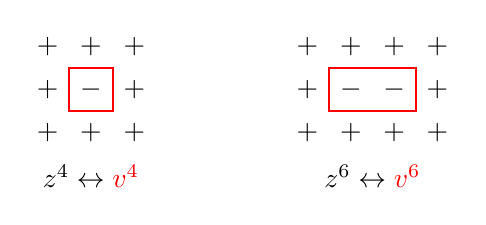
\begin{tikzpicture}[scale=0.55]
  \foreach \x/\y/\s in {0/0/+,1/0/+,2/0/+,0/1/+,1/1/-,2/1/+,0/2/+,1/2/+,2/2/+} \node at (\x,\y) {$\s$};
  \draw[red,thick] (0.5,0.5) rectangle (1.5,1.5);
  \node at (1,-1) {$z^4\leftrightarrow{\color{red}v^4}$};
  \begin{scope}[xshift=6cm]
  \foreach \x/\y/\s in {0/0/+,1/0/+,2/0/+,3/0/+,0/1/+,1/1/-,2/1/-,3/1/+,0/2/+,1/2/+,2/2/+,3/2/+} \node at (\x,\y) {$\s$};
  \draw[red,thick] (0.5,0.5) rectangle (2.5,1.5);
  \node at (1.5,-1) {$z^6\leftrightarrow{\color{red}v^6}$};
  \end{scope}
\end{tikzpicture}
\diagramcaption{One- and two-spin flips in the low-temperature expansion and the corresponding
closed polygons on the dual lattice in the high-temperature expansion.}
\end{diagram}

$T_c$ occurs at the point where the high-$T$ and low-$T$ expansions coincide, i.e.\ at $z = v$. Now
\begin{equation}
  v = \tanh K = \frac{e^K-e^{-K}}{e^K+e^{-K}} = \frac{1-e^{-2K}}{1+e^{-2K}} = \frac{1-z}{1+z},
  \qquad\text{inverse:}\quad z = \frac{1-v}{1+v}.
\end{equation}
So $z = v$ is the equation
\begin{equation}
  z = \frac{1-z}{1+z},\qquad\text{i.e.}\quad z+z^2 = 1-z;\qquad z^2+2z-1 = 0 .
\end{equation}
Solutions: $z = (1/2)\left[-2\pm 2\sqrt2\right]$, i.e.\ $z = -1\pm\sqrt2$. The solution with a $-$
sign gives $z<0$, unphysical, so the unique physical solution is
\begin{equation}
  z = z_c = -1+\sqrt2 ;
\end{equation}
now $z = e^{-2K}$, so $e^{-2K_c} = \sqrt2-1$, so $-2K_c = \ln(\sqrt2-1)$, i.e.\
$K_c = -(1/2)\ln(\sqrt2-1) = +(1/2)\ln\left(1/(\sqrt2-1)\right)$
\begin{equation}
  \Rightarrow\quad K_c = \frac{1}{2}\ln(\sqrt2+1) = 0.4407 .
\end{equation}
Since $K = \beta J = J/(\kB T)$, this yields the result
\begin{equation}
  \kB T_c = \frac{J}{(1/2)\ln(\sqrt2+1)} = 2.269\,J .
\end{equation}
This derivation was obtained by Kramers and Wannier in 1941, before the Onsager calculation of the
free energy of the (zero-field) Ising model on the square lattice (which was published in 1944). Of
course, from a knowledge of the ($H = 0$) free energy, one can determine $T_c$, but the
Kramers--Wannier derivation of $T_c$ shows how one can sometimes determine some properties of a
stat.\ mech.\ system exactly even without knowing the free energy.
